\chapter{Evaluation}
% This is where Assessors will be looking for signs of success and for evidence of thorough and systematic evaluation as discussed in Section 8.3. Sample output, tables of timings and photographs of workstation screens, oscilloscope traces or circuit boards may be included. A graph that does not indicate confidence intervals will generally leave a professional scientist with a negative impression.
% As with code, voluminous examples of sample output are usually best left to appendices or omitted altogether.
% There are some obvious questions which this chapter will address. How many of the original goals were achieved? Were they proved to have been achieved? Did the program, hardware, or theory really work?
% Assessors are well aware that large programs will very likely include some residual bugs. It should always be possible to demonstrate that a program works in simple cases and it is instructive to demonstrate how close it is to working in a really ambitious case.

% ~2,000 words

\begin{itemize}
    \item Permutation testing on features/labels or both, measuring $r$, $r^2$
    \item Plot with test set performance of best GCN and best GAT model
    \item Compare with literature on brain age estimation? (i.e. this model is quite poor)
    \item Robustness of the graphs: adding percentage noise to nodes and removing percentage edges
\end{itemize}

\section{Model ranking and selection}
Following the \texttt{wandb} hyperparameter tuning process described in Section~\ref{section:training-procedure}, the models were selected according to the following procedure (applied separately to the GCN and GAT model families):
\begin{enumerate}
    \item First, the models were ranked by ascending average MSE. The model with the lowest average MSE was chosen as the reference model.
    \item All models whose 1 standard deviation interval from their MSE did not overlap with the 1 standard deviation interval of the reference MSE were filtered out.
\end{enumerate}

The performance of the best-scoring models selected by the above procedure are shown in Figures~\ref{figure:gcn-rank} and~\ref{figure:gat-rank} for the GCN and GAT model families respectively. The hyperparameters for each of the shortlisted models are listed in Appendix ?.

\begin{figure}[]
    \centering
    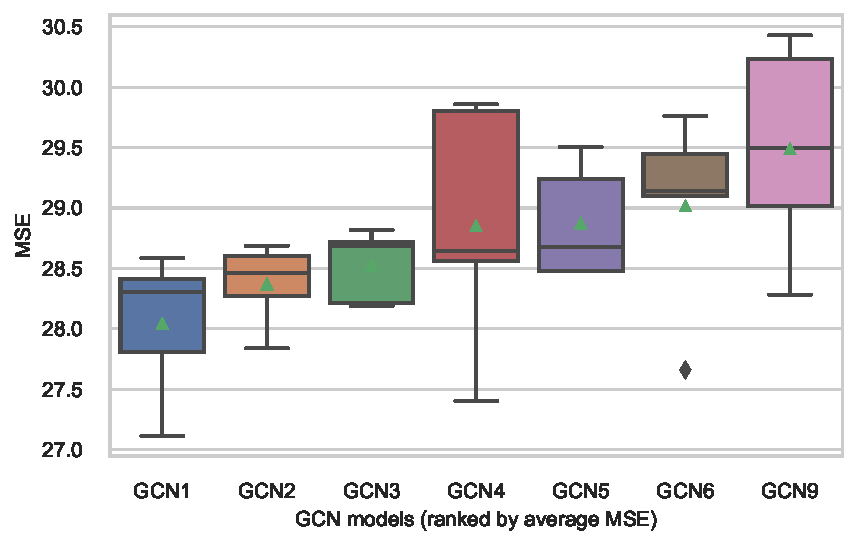
\includegraphics[width=\textwidth]{gcn_model_selection.pdf}
    \caption{Highest scoring population graph and GCN model parameter combinations.}\label{figure:gcn-rank}
\end{figure}

\begin{figure}[]
    \centering
    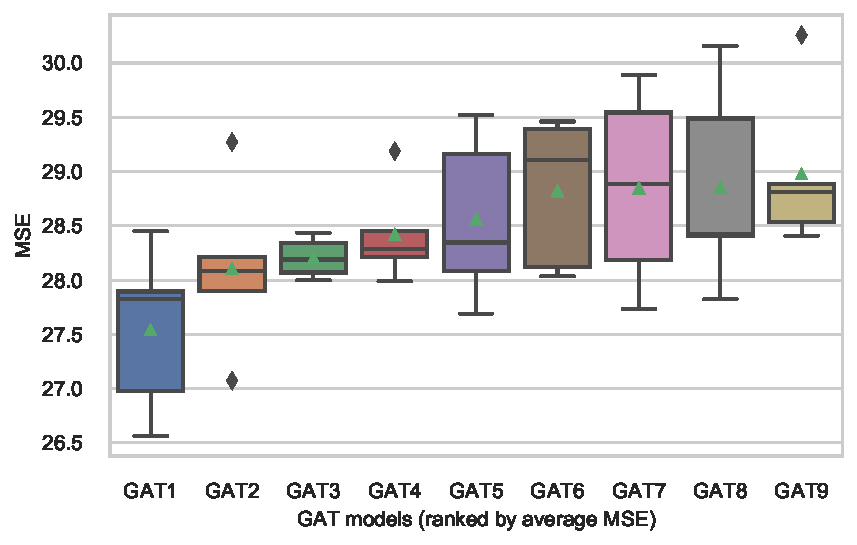
\includegraphics[width=\textwidth]{gat_model_selection.pdf}
    \caption{Highest scoring population graph and GAT model parameter combinations.}\label{figure:gat-rank}
\end{figure}

Although both best-ranked models (GCN1 and GAT1) seem to have relatively high variance, they still look the most promising and therefore have been selected for the evaluation procedure. Their population graph and GNN architecture hyperparameters are listed in Table~\ref{table:best-hyperparameters}.

\begin{table}[]
    \caption{Best performing population graph and GNN model parameter combinations after model selection process.}\label{table:best-hyperparameters}
    \centering
    \small
    \begin{tabular}{p{0.3\textwidth}p{0.3\textwidth}p{0.3\textwidth}}
        \hline
    \textbf{Hyperparameter} & \textbf{GCN1} & \textbf{GAT1} \\  \hline
        Similarity feature set & \texttt{FI}, \texttt{FTE}, \texttt{ICD10}, \texttt{MEM}, \texttt{SEX} & \texttt{FI}, \texttt{ICD10}, \texttt{MEM}, \texttt{SEX} \\
        Similarity threshold & 0.9 & 0.8 \\ \hline
        Layer sizes & [1024, 512, 512, 256, 256, 1] & [2048, 1024, 512, 256, 128, 1] \\
        \# convolutional layers & 5 & 2 \\
        Dropout & $3.22 \times 10^{-1}$ & $3.14 \times 10^{-3}$ \\
        Learning rate & $6.98 \times 10^{-3}$ & $1.34 \times 10^{-2}$ \\
        Weight decay & $1.31 \times 10^{-2}$ & $6.05 \times 10^{-4}$ \\ \hline
\end{tabular}
\end{table}


% \section{Comparison against existing benchmarks}

% Compare to the Kaufmann et al.'s \textit{xgboost} approach \cite{kaufmann2019} ($r \sim 0.93$); and the other package that was cited in the same paper.
% Possibly compare to other non-graph (relatively baseline) (neural network) architectures, e.g. ElasticNet, MLP,...

